% Author: Dominik Harmim <harmim6@gmail.com>

\documentclass[10pt, hyperref={unicode}, aspectratio=169]{beamer}

\usepackage{newcent}
\usepackage[utf8]{inputenc}
\usepackage[czech, british]{babel}
\usepackage[T1]{fontenc}
\usepackage{listings}
\usepackage{appendixnumberbeamer}

\lstset{
    basicstyle=\ttfamily,
    keywordstyle=\color{blue},
    language=C,
    tabsize=2,
    escapeinside={<@}{@>},
    frame=shadowbox
}


\usetheme{FIT}

\title{Static Analysis Using Facebook Infer to Find Atomicity~Violations}

\author{\texorpdfstring{%
    Dominik Harmim \\
    \footnotesize{Supervisor: prof. Ing. Tomáš Vojnar, Ph.D.}
}{Dominik Harmim, Supervisor: prof. Ing. Tomáš Vojnar, Ph.D.}}

\institute{%
    xharmi00@stud.fit.vutbr.cz \\
    Brno University of Technology, Faculty of Information Technology
}

\date{\today}


\begin{document}


\section{Title page}
\frame[plain]{\titlepage}


\section{Motivation}
\begin{frame}[fragile]{Motivation}
    \begin{itemize}
        \item
            \alert{Atomicity}: property that a series of operations should be
            indivisible.

            \smallskip

            \begin{itemize}\setlength\itemsep{1em}
                \item
                    Often required in \emph{concurrent programs}.

                \item
                    Violation may cause \emph{significant damage}.
            \end{itemize}
    \end{itemize}

    \medskip
    \begin{columns}
        \begin{column}{.6 \linewidth}
            \centering

            \begin{lstlisting}
void replace(int *array, int a, int b) {
    int i = <@\texttt{\textbf{index\_of}}@>(array, a);
    if (i >= 0) <@\texttt{\textbf{set}}@>(array, i, b);
}
            \end{lstlisting}
        \end{column}

        \begin{column}{.4 \linewidth}
            \centering

            \texttt{\textbf{index\_of}} and \texttt{\textbf{set}}
            should be \alert{executed atomically}

            \medskip

            {\footnotesize
                The index may be \emph{outdated} because of
                a~\emph{concurrent modification} of an array.
            }
        \end{column}
    \end{columns}
    \medskip

    \begin{itemize}
        \item
            \emph{Shortcomings} of current analysers for finding
            \alert{atomicity violations}:

        \smallskip

        \begin{itemize}\setlength\itemsep{1em}
            \item
                a~high rate of \emph{false positives},

            \item
                \emph{scalability},

            \item
                \ldots
        \end{itemize}
    \end{itemize}
\end{frame}


\section{Facebook Infer}
\begin{frame}{Facebook Infer}
    \begin{columns}
        \begin{column}{1 \linewidth}
            \begin{itemize}
                \item
                    An open-source \alert{static analysis framework}
                    for \emph{interprocedural analyses}.

                    \smallskip

                    \begin{itemize}\setlength\itemsep{1em}
                        \item
                            Based on \alert{abstract interpretation}.
                    \end{itemize}
            \end{itemize}
        \end{column}

        \hfill
    \end{columns}

    \begin{columns}
        \begin{column}{.55 \linewidth}
            \begin{itemize}\setlength\itemsep{2em}
                \item
                    \alert{Highly scalable}.

                    \smallskip

                    \begin{itemize}\setlength\itemsep{1em}
                        \item
                            Follows principles of \emph{compositionality}.

                        \item
                            Computes function \emph{summaries} bottom-up
                            on call trees.
                    \end{itemize}

                \item
                    Supports Java, C, C++ and Objective-C.
            \end{itemize}
        \end{column}

        \begin{column}{.45 \linewidth}
            \begin{center}
                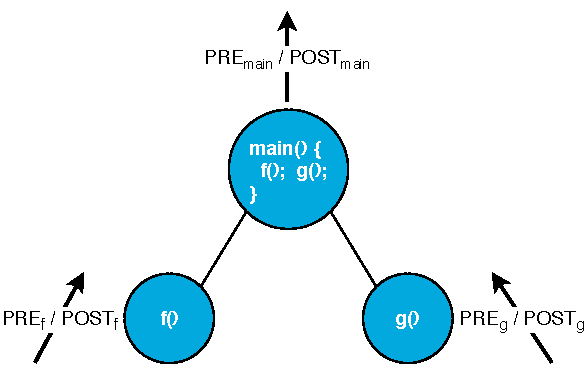
\includegraphics[width=1 \linewidth]{img/infer.pdf}
            \end{center}
        \end{column}
    \end{columns}
\end{frame}


\section{Atomer: Proposed Atomicity Violations Checker}
\begin{frame}{Atomer: Proposed Atomicity Violations Checker}
    \begin{itemize}\setlength\itemsep{3em}
        \item
            \alert{Atomicity violations} for \emph{sequences of
            functions}.

        \item
            Sequences executed \emph{atomically once} should be
            executed \emph{always atomically}.

        \item
            Targets \emph{C/C++} programs that use \emph{PThread locks}.
    \end{itemize}
\end{frame}


\section{Atomer: Two Phases of the Analysis}
\begin{frame}[fragile]{Atomer: Two Phases of the Analysis}
    \begin{columns}
        \begin{column}[T]{.5 \linewidth}
            \centering

            \begin{enumerate}
                \item
                    Detection of \alert{atomic sequences}.
            \end{enumerate}

            \begin{itemize}\setlength\itemsep{1em}
                \item
                    Working with \emph{sequences of calls}.

                \item
                    Only \emph{first occurrences} remembered to assure
                    a~termination.
            \end{itemize}

            \begin{lstlisting}
void f(int *array) {
    <@\texttt{\textcolor{red}{\textbf{pthread\_mutex\_lock}}}@>(&lock);
    int i = <@\texttt{\textbf{index\_of}}@>(array, 42);
    if (i >= 0) <@\texttt{\textbf{set}}@>(array, i, 3);
    <@\texttt{\textcolor{red}{\textbf{pthread\_mutex\_unlock}}}@>(&lock);
}
            \end{lstlisting}

            \alert{\textbf{\texttt{
                summary\textsubscript{f}: \{(index\_of, set)\}
            }}}
        \end{column}

        \begin{column}[T]{.5 \linewidth}
            \centering

            \begin{enumerate}\setcounter{enumi}{1}
                \item
                    Detection of \alert{violations}.
            \end{enumerate}

            \begin{itemize}
                \item
                    Split to sets of \emph{pairs of subsequent calls}
                    without and with a~lock.
            \end{itemize}

            \begin{lstlisting}
void g(int *array) {
    int i = <@\texttt{\textbf{index\_of}}@>(array, 66);
    if (i >= 0) <@\texttt{\textbf{set}}@>(array, i, 5);
}
            \end{lstlisting}

            \alert{\textbf{\textsc{Atomicity Violation!}}}
        \end{column}
    \end{columns}
\end{frame}


\section{Experimental Evaluation}
\begin{frame}{Experimental Evaluation}
    \begin{columns}
        \begin{column}{.5 \textwidth}
            \begin{itemize}\setlength\itemsep{1.5em}
                \item
                    The \alert{correctness} was verified
                    on \emph{hand-crafted} programs.

                \item
                    Evaluated on \emph{real-life low-level concurrent}
                    programs from Debian GNU Linux.

                    \smallskip

                    \begin{itemize}\setlength\itemsep{1em}
                        \item
                            Analysed thousands of lines of code.

                        \item
                            So far quite some false alarms and
                            limited scalability.
                    \end{itemize}
            \end{itemize}
        \end{column}

        \begin{column}{.5 \textwidth}
            \def\arraystretch{1.3}

            \begin{tabular}{lrr}
                & \textbf{Lines of} & \alert{\textbf{Atomicity}} \\
                \textbf{Program} & \textbf{Code}
                    & \alert{\textbf{Violations}} \\ \hline

                glfw 2.7.9 & 10,230 & 13 \\ \hline
                alsa-utils 1.1.0 & 7,735 & 1 \\ \hline
                c-icap 0.4.2 & 24,923 & 174 \\ \hline
                npth 1.2 & 1,593 & 26 \\ \hline
                rt-tests 0.96 & 1,795 & 0 \\ \hline
                sslsplit 0.4.11 & 22,457 & 344 \\ \hline
            \end{tabular}
        \end{column}
    \end{columns}
\end{frame}


\section{Summary}
\begin{frame}{Summary}
    \textbf{The \emph{static analyser} for finding \alert{atomicity
    violations}:}
    \medskip
    \begin{itemize}\setlength\itemsep{.5em}
        \item
            \emph{Proposed} and \emph{implemented} as
            a~module of \alert{Facebook Infer}.

        \item
            Successfully \emph{tested} and \emph{experimentally
            evaluated}.

        \item
            The preliminary results were presented at \emph{Excel@FIT'19}.
    \end{itemize}

    \bigskip

    \textbf{Future goals:}
    \medskip
    \begin{itemize}\setlength\itemsep{.5em}
        \item
            Increase the \alert{accuracy}.

            \begin{itemize}
                \item
                    By, e.g., considering \emph{function parameters}.
            \end{itemize}

        \item
            Enhance the \alert{scalability}.

           \begin{itemize}
               \item
                    To be able to analyse more extensive programs.
           \end{itemize}

        \item
            Create a~\emph{Pull Request} to the \texttt{master}
            branch of Facebook Infer.
    \end{itemize}
\end{frame}


\appendix


\section{Otázky oponenta}
\begin{frame}{Otázky oponenta}
    \textbf{Diskutujte obtížnost rozšíření analyzátoru Atomer o~podporu
    \emph{formálních parametrů} funkcí a~\emph{návratových hodnot}.}
    \vspace{2em}
    \begin{itemize}\setlength\itemsep{1.5em}
        \item
            Využití: \alert{rozlišení kontextu} volaných
            funkcí.

        \item
            Vhodná charakterizace hodnot \emph{staticky}
            a~\emph{abstraktně}.

            \smallskip

            \begin{itemize}\setlength\itemsep{1em}
                \item
                    Možnost použít \alert{syntaktické
                    \uv{access paths}} (lokace na haldě).

                \item
                    K~bližšímu rozlišení nutno použít
                    \emph{ukazatelové analýzy}.
            \end{itemize}
    \end{itemize}
\end{frame}


\end{document}
